\chapter[SCP-150 义肢寄生虫]{
    SCP-150 The Prosthetic Parasite\\
    SCP-150 义肢寄生虫
}

\label{chap:SCP-150}

\begin{figure}[H]
    \centering
    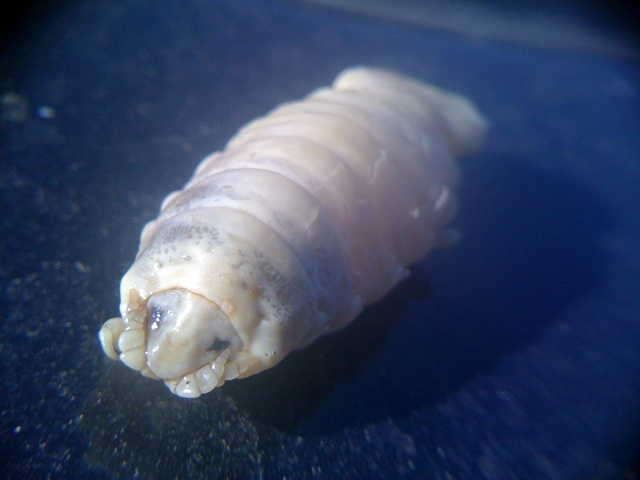
\includegraphics[width=0.5\linewidth]{images/SCP.150.jpg}
    \caption*{SCP-150 的一个样本}
\end{figure}

\bb{项目编号:}SCP-150

\bb{项目等级:}Euclid

\bb{特殊收容措施:}SCP-150应该被放置于一个位于生物研究区域12{[}原文:Bio-Research Area-12]的控制收容小室中。为了防止感染,所有人员在进入小室时需要穿戴4级生化装备。不需要更深入的收容章程。

\bb{描述:}SCP-150似乎是一种\ii{Cymothoa exigua}(缩头鱼虱),但是对\ii{Homo sapiens}同样有效。一经接触,项目将会把自己深深地埋入寄主的肉体之中。在48小时之内距离感染处最近的肢体将会被转换成一种像外甲壳一样的几丁质附肢。这些外甲壳完全由与SCP-150一致的物质组成。寄主能像控制正常的肢体一样控制这些肢体,这归因于在寄主和寄生虫之间的一种高级神经肌肉接触。寄生虫从被同化的血管中汲取营养。首先是手臂中的前肢和桡骨动脉,然后是位于腿部的股骨动脉。

感染的第二阶段大约在感染7天后发生。寄主报告感觉到了不寻常的声音,催促他们进行一种将会导致寄生肢体脱落的行为。从寄主脱落后,附肢表现得十分像一个剥落的体外甲壳。复数的寄生虫从这个茧中显露并搜寻最近的寄主,因而继续进行循环。在██\%的事件中,孵化出的寄生虫回到了他们原始的寄主。这将会继续直到原始寄主的所有肢体都已经被感染。一旦寄主所有的附肢都已经被感染且分离,复数的SCP-150实体将会探查寄主的躯干。这些样本将让自己附着在肺动脉、主动脉和颈动脉上。寄主的胸部将会隆起至原来尺寸的 ███\%。此时,在██和███中的SCP-150样本将从寄主的胸腔显露。第三阶段的感染有着100\%的致死率。
